The event panel presents the user with a drop-down menu with a list of
available event applications. Event applications are applications
that, given the building and user supplied data inputs, will generate
a list of events (i.e., typically time-dependent loads that represent natural disasters) for the building. The following options
are available in the drop-down menu:

\begin{enumerate}
\item Multiple Existing SimCenter Events (\Cref{subsec:multiple_existing})
\item Multiple PEER Events (\Cref{subsec:multiple_peer})
\item Hazard Based Event (\Cref{subsec:hazard_based})
\item Stochastic Ground Motion (\Cref{subsec:stochastic_motions})
\item Site Response (\Cref{subsec:site_response})
\item User Application (\Cref{subsec:user_event})
\end{enumerate}

\subsection{Multiple Existing}
\label{subsec:multiple_existing}
This panel is provided for the user to specify multiple existing SimCenter
event files.  If more than one event is specified it is done to
provide the UQ engine with a discrete set of events to choose
from\textemdash it is not done with the intention of specifying that
one event follows another.  The panel presented to the user
is shown in \Cref{fig:SC_event_panel}.

\begin{figure}[!htbp]
  \centering {
    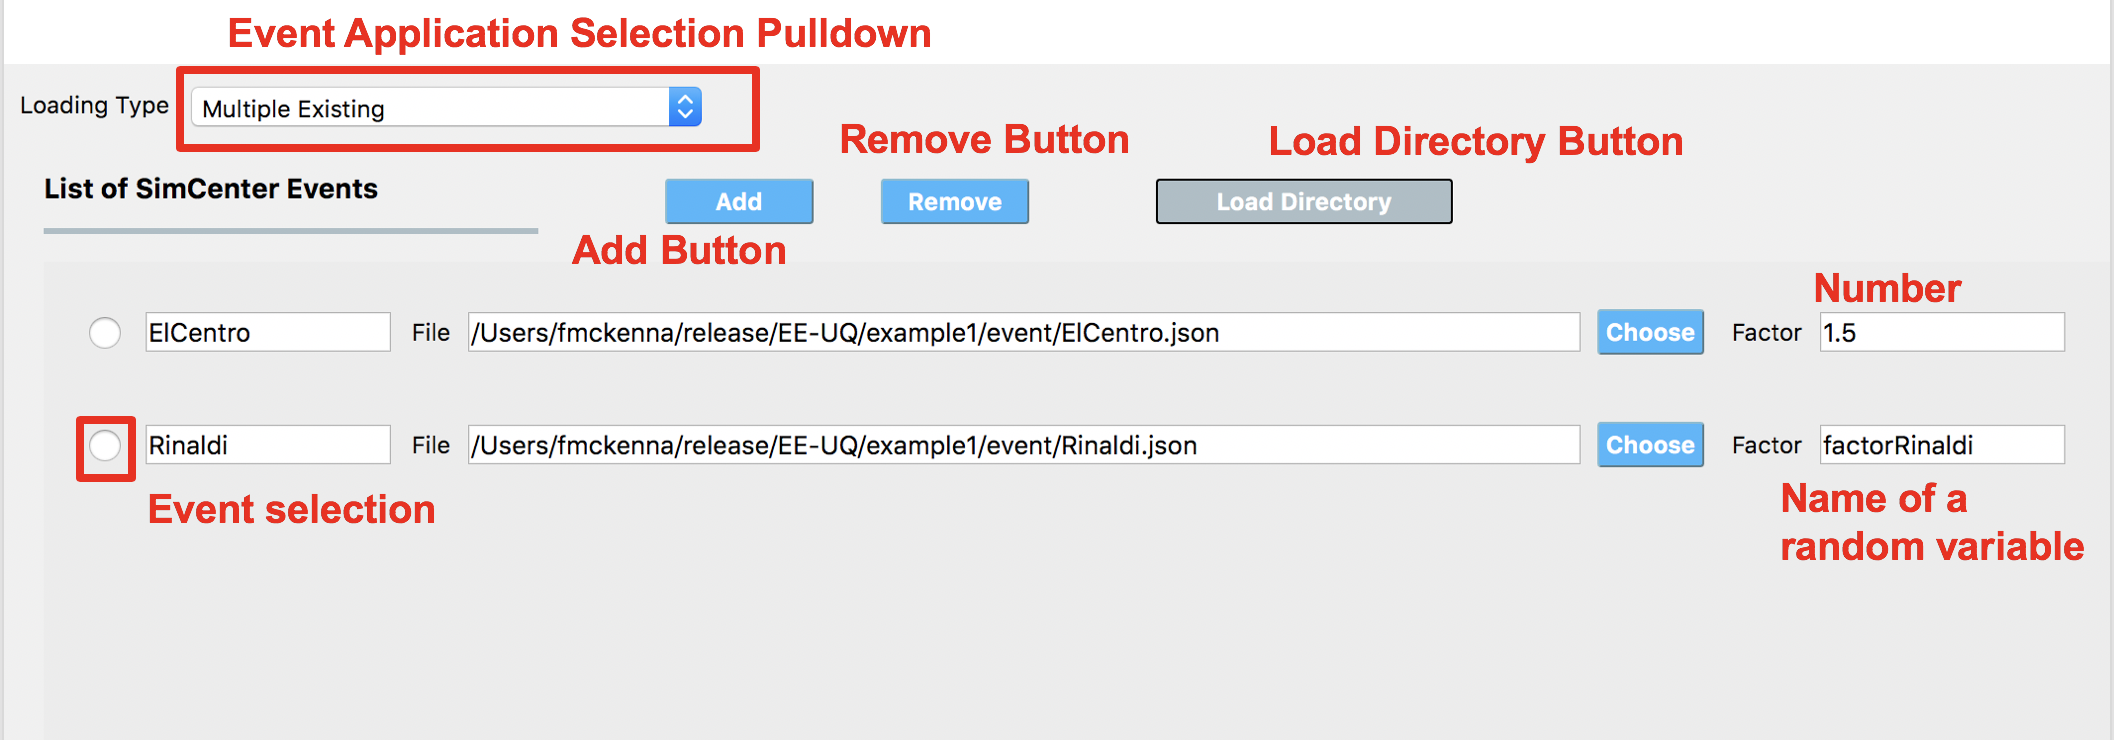
\includegraphics[width=0.8\textwidth]
    {usage/figures/multipleExisting.png} }
  \caption{Multiple Existing (SimCenter) Events }
  \label{fig:SC_event_panel}
\end{figure}

Use the \texttt{Add} button to add a new event. This adds an empty
event to the panel. Pressing the button multiple times will keep
adding events to the panel. \Cref{fig:SC_event_panel} shows the state after
the button has been pressed twice, and data entered to load the El Centro
and Rinaldi Events.

The path to the event file can be entered manually, or using the \texttt{Choose} button for convenience. Pushing the button brings up a typical file search screen. By default, a scale factor of 1.0 is assigned to the event.  The user
can change this to another floating point value (DO NOT USE INTEGER), and they can define the scale factor as a random variable by
entering a variable name, such as \texttt{factorRinaldi} for the second event in \Cref{fig:SC_event_panel}.

Note: the name of the random variable must not start with a number, or contain any spaces or special characters, such as -, +, \%, etc.

The \texttt{Remove} button is used to remove events. To remove an
event, the user must first select events they wish to remove,
which is done by clicking in the small circle at the left side of the event frame. All of the selected events are removed when the \texttt{Remove} button is pressed.

The \texttt{Load Directory} button provides a convenient method to load multiple events. All event files shall first
be placed into the same folder. We recommend to put the files in a folder of their own, with no other files besides the earthquake events in it. After pressing the \texttt{Load Directory} button, the user will be able to choose the directory that contains the files, and the
application will load all event files (i.e., every file with a \texttt{.json} 
extension) into the widget automatically. 

Initially, every
event will be given a load factor of 1.0. Load factors can be assigned automatically by preparing a \texttt{Records.txt} file in the directory with the events. Each line in the \texttt{Records.txt} shall represent one event file, and contain two comma separated values: the event file name and the desired scale factor. The application will open that file automatically and assign the prescribed load factors to the events. Using a \texttt{Records.txt} file also allows users to load only a subset of the events from a folder by listing only those in the file. An example \texttt{Records.txt} is shown below:

\begin{verbatim}
ElCentro.json,1.5
Rinaldi.json,2.0
\end{verbatim}

Random Variables: Scale factors can be defined as being random variables by entering a string in the factor field. The variable name entered will appear as a Random Variable in the UQ panel and the user must specify its distribution there. If multiple
events are specified, the event itself will be also be treated as a random
variable, with each event being part of the discrete set of possible
events. For discrete events the user does not define a distribution, this is done automatically.


\subsection{Multiple PEER Event}
\label{subsec:multiple_peer}
This event option is provided for the user to specify multiple existing
\href{http://peer.berkeley.edu}{PEER} ground
motion files.  For PEER events, the user is required to specify the
individual components for the EVENTS.  The \texttt{Add/Remove} buttons
at the top are to create and remove an event, as
per \Cref{subsec:multiple_existing}. For the PEER events, the user
specifies components acting in the individual degree-of-freedom
directions.  The \texttt{+} and \texttt{-} buttons add and remove
components with remove removing all components selected. Each
component in a PEER event can have their own scale factor, again a
number or a random variable.

\begin{figure}[!htbp]
  \centering {
    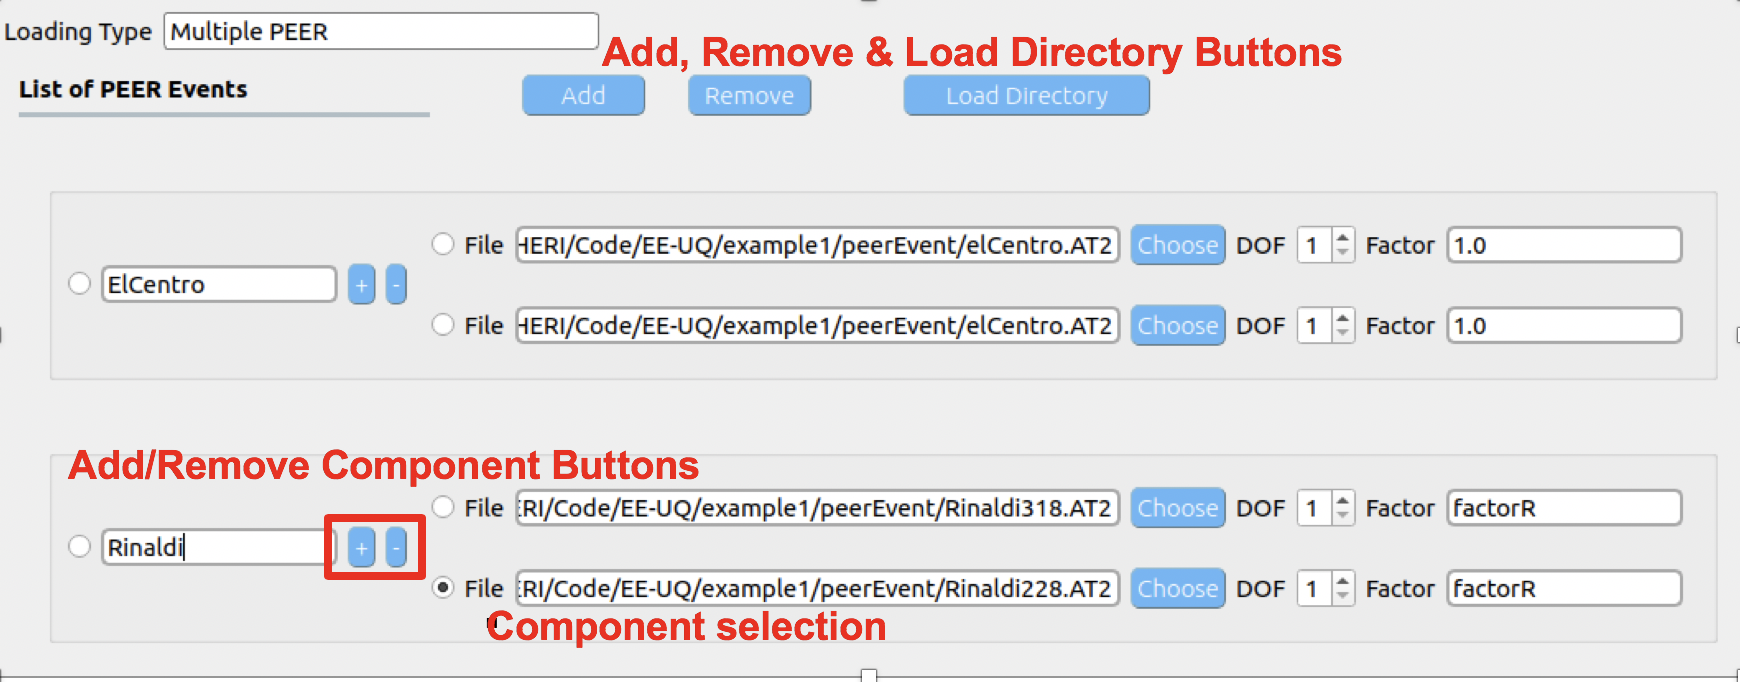
\includegraphics[width=0.8\textwidth]
    {usage/figures/multiplePEER.png} }
  \caption{\texttt{Multiple PEER} loading type}
  \label{fig:figure6}
\end{figure}

If the user has multiple events to load, they can again place all the
PEER \texttt{.AT2} files into a separate folder and select
the \texttt{Load Directory} option. This will allow the user to select
a directory. Once selected, all \texttt{.AT2} files in that directory will be
loaded into the application. Similar to loading multiple SimCenter
events, should the user provide a file \texttt{Records.txt} in that
directory, the application will load all files in the list and set the
appropriate load factor. An example \texttt{Results.txt} file for multiple Peer
events is as shown below:

\begin{verbatim}
elCentro.AT2,1.5
Rinaldi228.AT2,2.0
Rinaldi318.AT2,2.0
\end{verbatim}

Random Variables: The user can, as mentioned, enter a string in the
factor field to specify that the factor is to be considered a random
variable. Subsequently, in the UQ panel the user must provide
information on the random variables distribution. Also, if multiple
events are specified, the event itself will be treated as a random
variable with each event being part of the discrete set of possible
events.


\subsection{Hazard Based Event}
\label{subsec:hazard_based}
The panel for this event application is as shown in
\autoref{fig:figure7}.  This application implements a scenario-based
(deterministic) seismic event.  In this panel the user specifies an
earthquake rupture (location, geometry and magnitude), a ground motion
prediction equation, a record selection database and the intensity
measure used for record selection.  In the backend, this application
relies on three other applications to perform seismic hazard analysis,
intensity measures simulation (to create a simulated target spectrum),
and ground motion record selection/scaling.  Users interested in
learning about those applications are referred to the documentation of
the
(\href{https://github.com/NHERI-SimCenter/GroundMotionUtilities/blob/master/Readme.md}{SimCenter
  ground motion utilities}).

\begin{figure}[!htbp]
  \centering {
    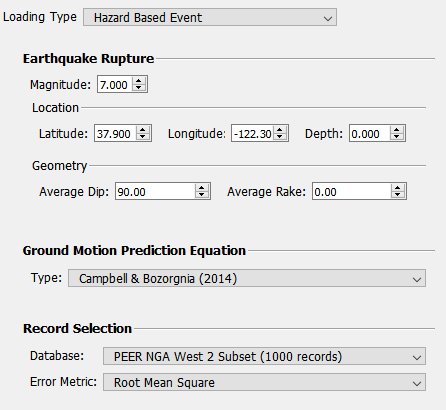
\includegraphics[width=0.8\textwidth]
    {usage/figures/hazardBased.png} }
  \caption{\texttt{Hazard Based Event} loading type}
  \label{fig:figure7}
\end{figure}


\subsection{Stochastic Ground Motion Model}
\label{subsec:stochastic_motions}
This option allows users to generate synthetic ground motions for a
target seismic event. In order to do so, the stochastic ground motion
model is selected from the drop-down menu, as shown
in \Cref{fig:stochastic_loading}. Depending on the model selected, the
user will be asked to enter values for a number of parameters that are
used to generate a seismic event. In the current release, users can
select between the model derived by Vlachos et
al. (2018) \cite{vlachos2018predictive} and the model developed by
Dabaghi \& Der Kiureghian (2014, 2017, 2018)
[\cite{dabaghi2014stochastic}, \cite{dabaghi2017stochastic}, \cite{dabaghi2018simulation}]. Additionally,
users can provide a seed for the stochastic motion generation if they
desire the same suite of synthetic motions to be generated on multiple
occasions.  If the seed is not specified, a different realization of
the time history will be generated for each run. The backend
application that generates the stochastic ground motions relies
on \texttt{smelt}, a modular and extensible C++ library for generating
stochastic time histories. Users interested in learning more about the
implementation and design of
\texttt{smelt} are referred to its
\href{https://github.com/NHERI-SimCenter/smelt}{GitHub repository}.

All input parameters can be specified as random variables by entering
a string in the parameter field. Please note that information for the
inputs that are identified as random variables needs to be provided in
the \texttt{UQ} tab.

\begin{figure}[!htbp]
  \centering {
    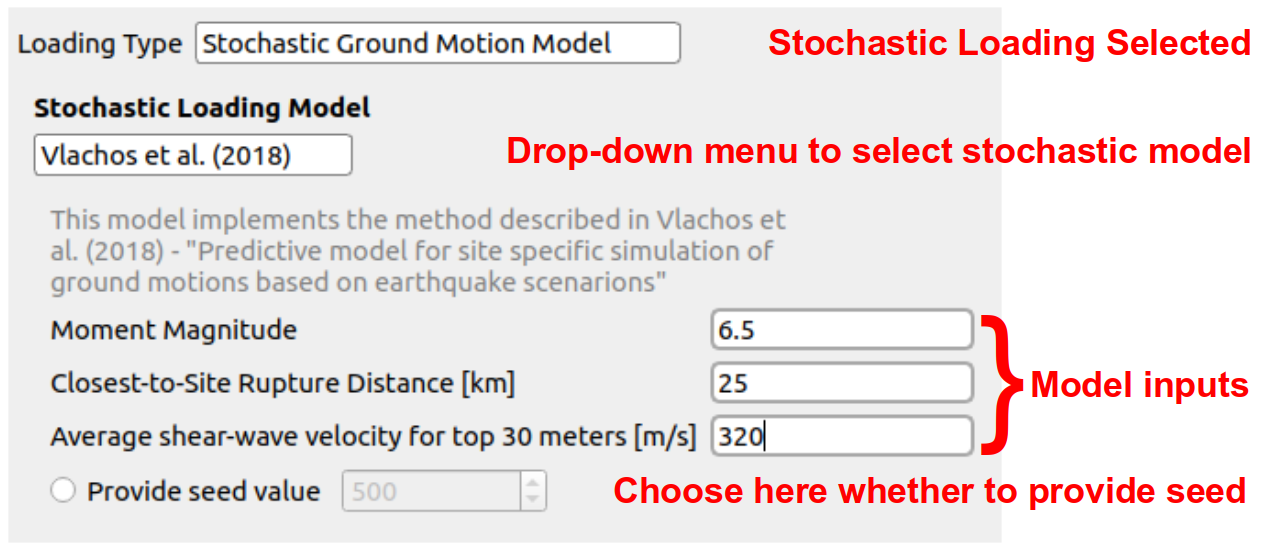
\includegraphics[width=0.8\textwidth]
    {usage/figures/stochastic_loading.png} }
  \caption{Stochastic Ground Motion Event}
  \label{fig:stochastic_loading}
\end{figure}


\subsection{Site Response}
\label{subsec:site_response}
The panel for this event application is as shown in \Cref{fig:s3hark0}. 
This application does effective free-field site response analysis of a soil column.
In this panel the user specifies a ground motion at the bottom of the column. 
With soil layer properly defined, the motion at the ground surface will be given at the end of the analysis.
\begin{figure}[!htbp]
  \centering {
    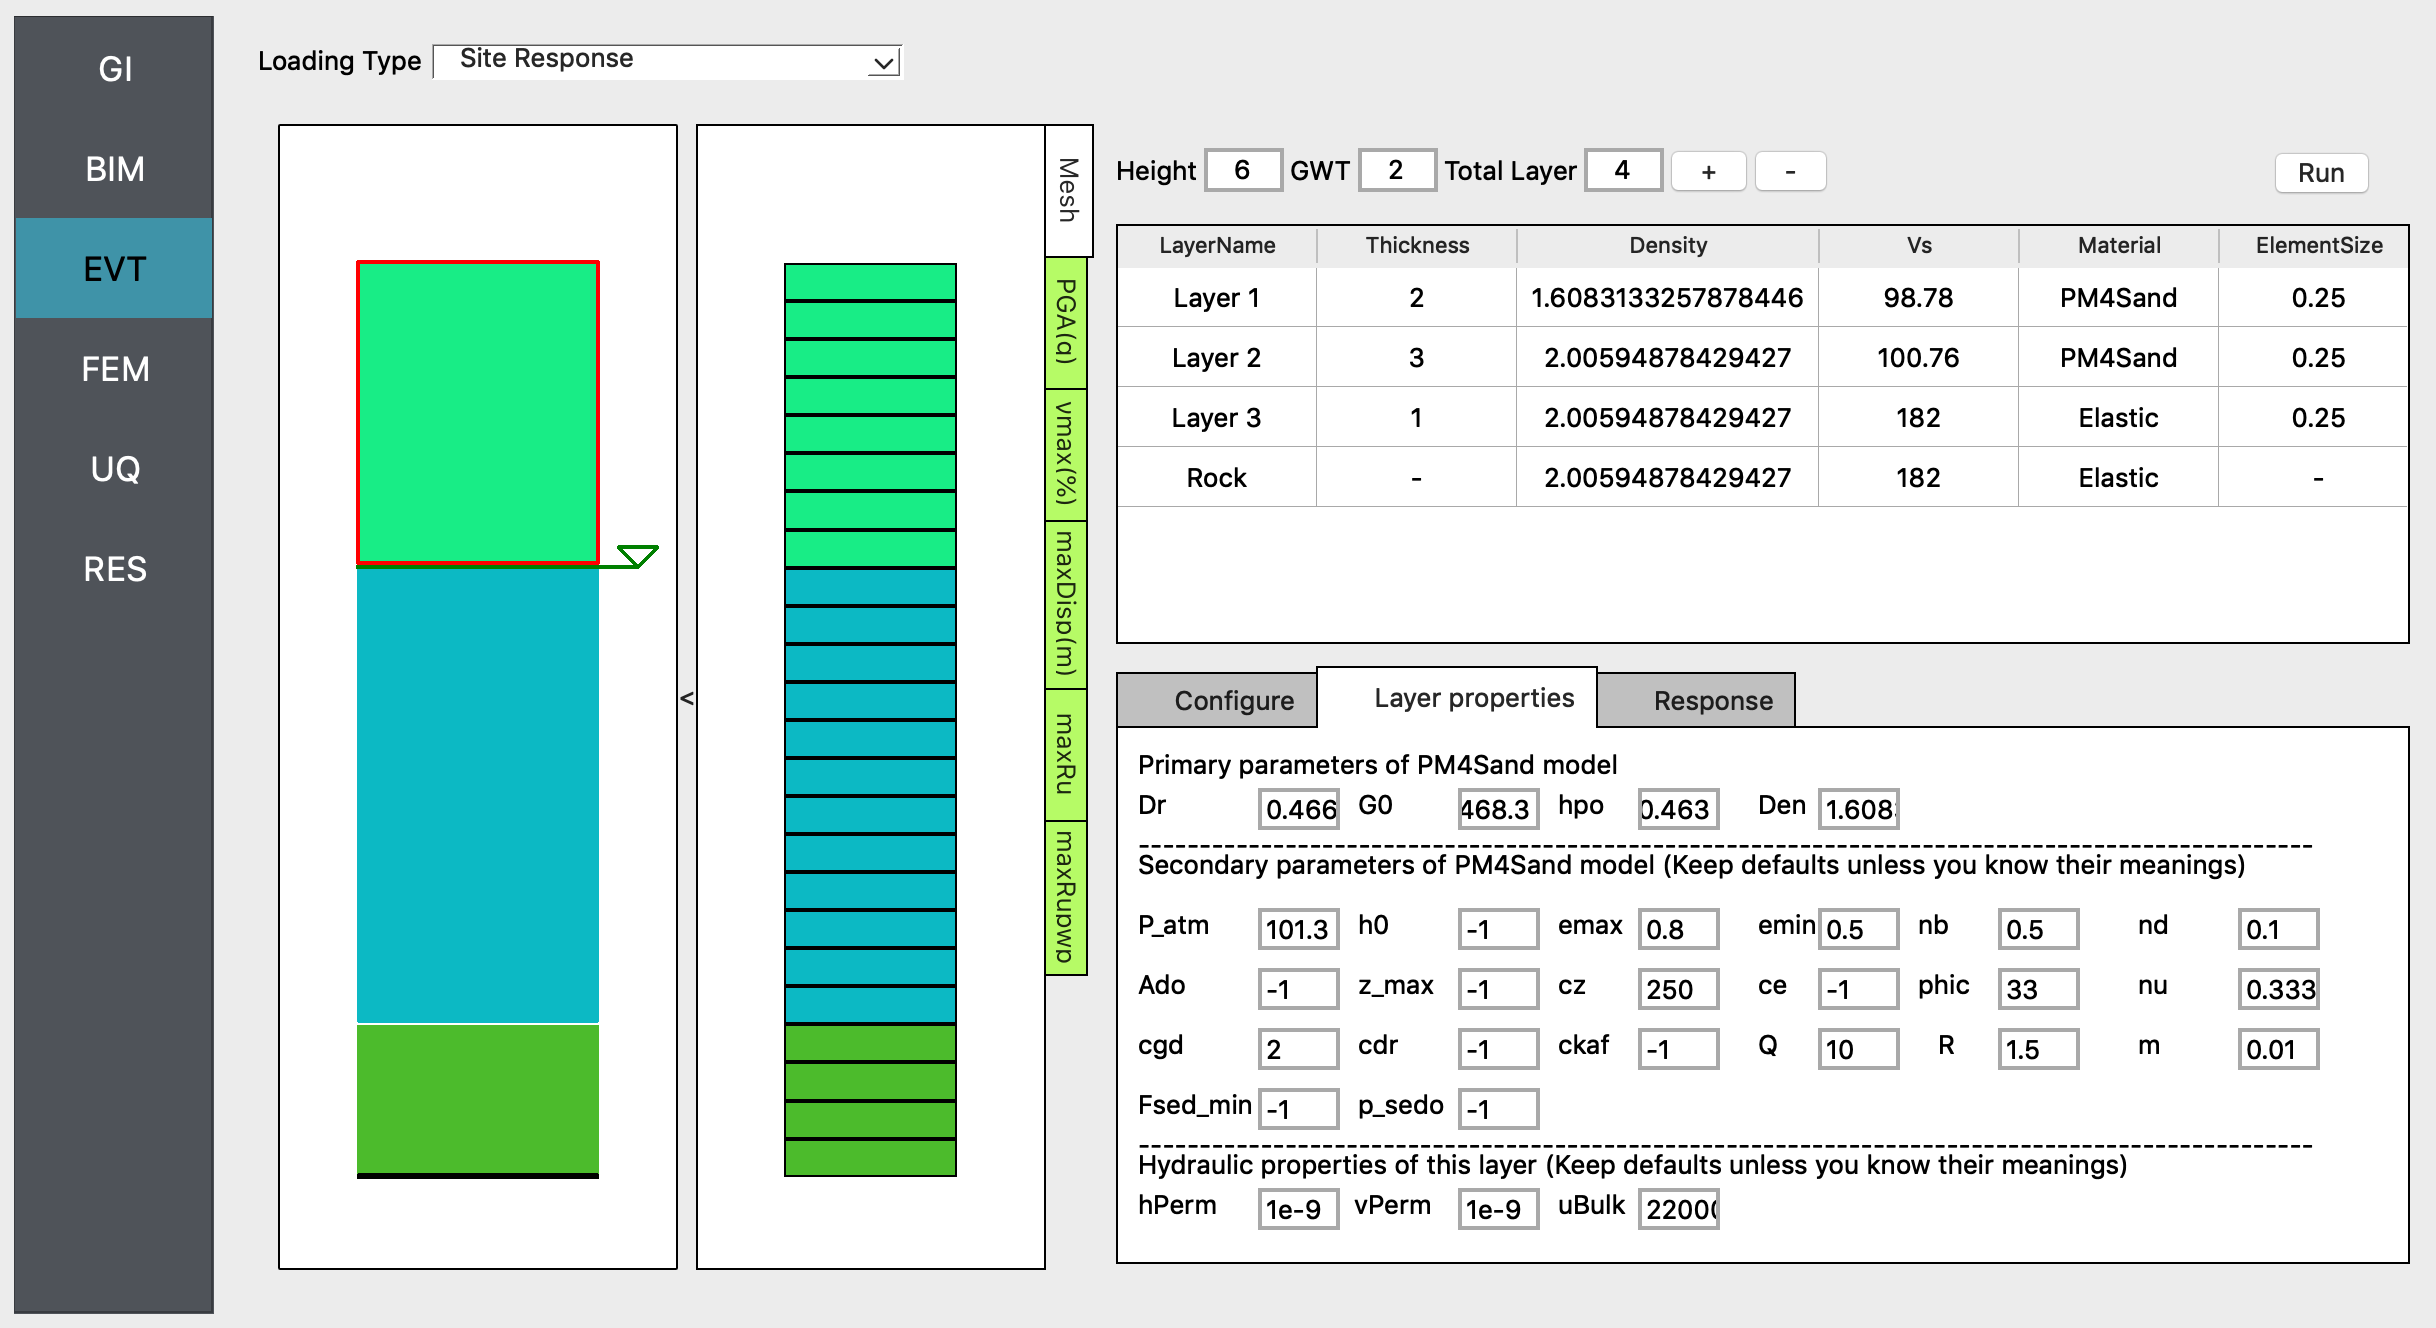
\includegraphics[width=0.8\textwidth]
    {usage/figures/s3hark0.png} }
  \caption{s$^3$hark}
  \label{fig:s3hark0}
\end{figure}

The UI of s$^3$hark is shown in \Cref{fig:s3hark1}.
There are two graphics shown in the left of the panel. The first one is the soil column graphic, 
which shows a visualization of the soil column.
The second one is the mesh and profile graphic, 
which shows the finite element mesh and profile plots.
On the right of the panel are operation area, soil design table, configure tab, layer property tab and response tab. 


\begin{figure}[!htbp]
  \centering {
    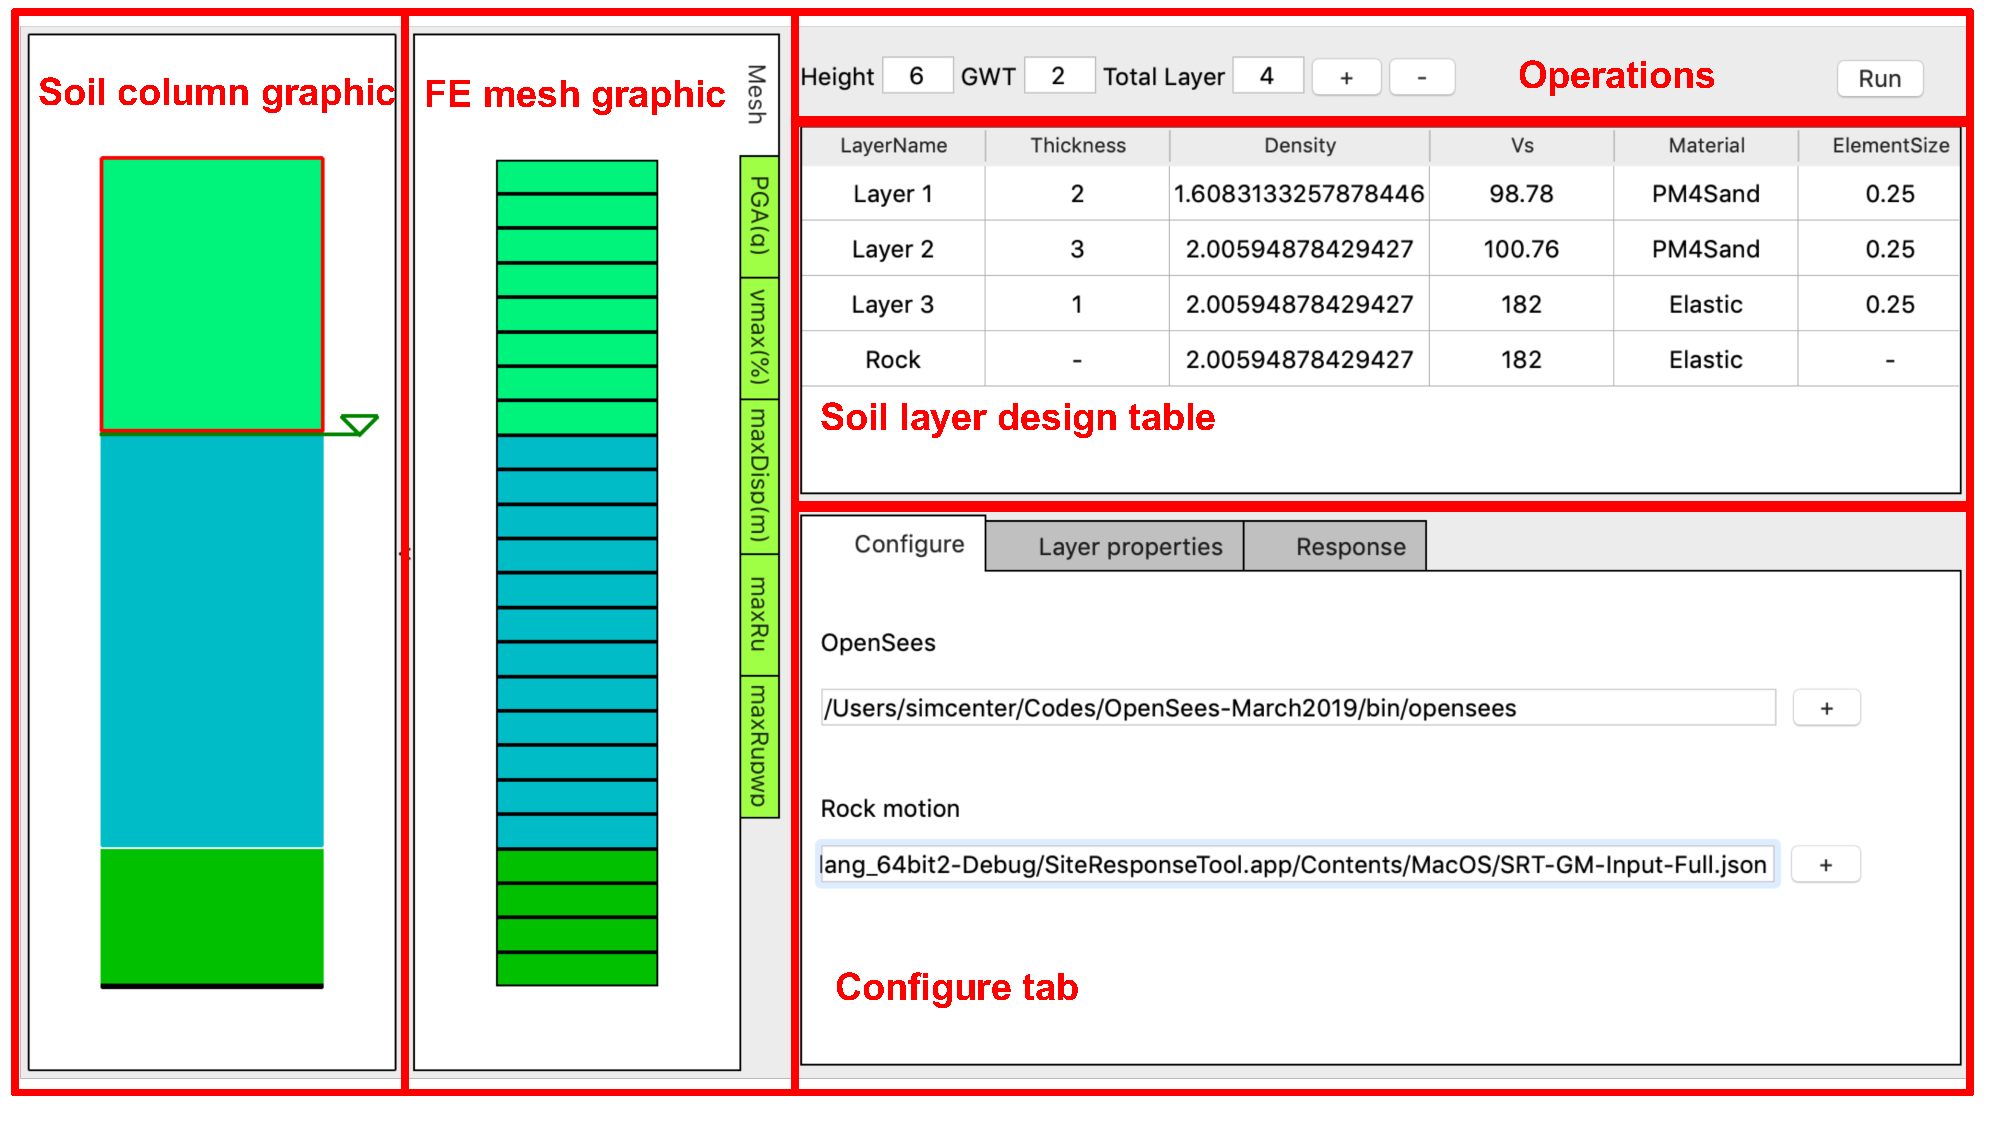
\includegraphics[width=0.8\textwidth]
    {usage/figures/s3hark1.pdf} }
  \caption{s$^3$hark - Panels}
  \label{fig:s3hark1}
\end{figure}

In the operation area as shown in \Cref{fig:s3hark2}, click the plus button to add a layer and the minors button to delete a selected layer. 
Change the ground water table in the GWT input field. 
In the configure tab, path of OpenSees executable and rock motion file need to be specified.
A click on the run button will start the finite element analysis.


\begin{figure}[!htbp]
  \centering {
    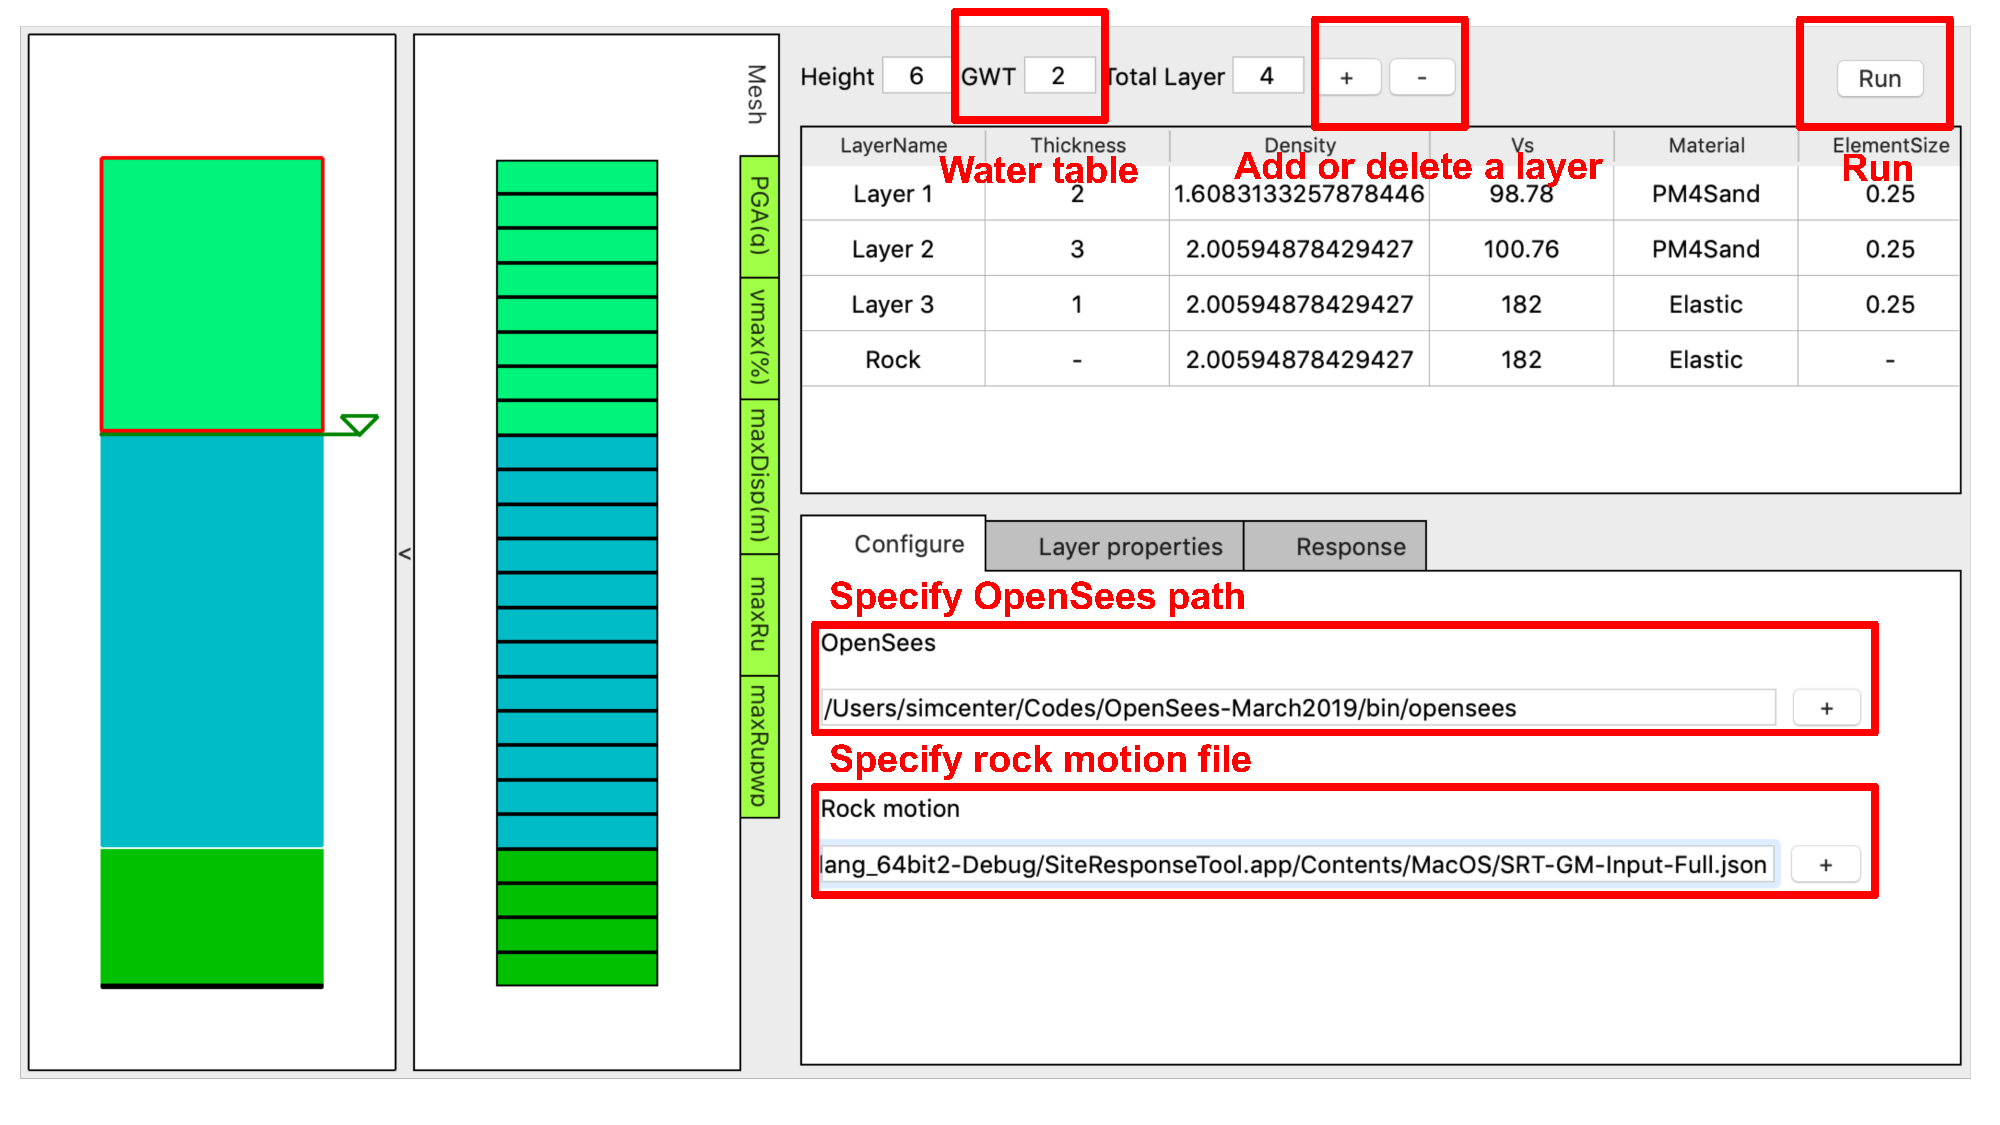
\includegraphics[width=0.8\textwidth]
    {usage/figures/s3hark2.pdf} }
  \caption{s$^3$hark - Configurations and Operations }
  \label{fig:s3hark2}
\end{figure}

Either click on the soil column or the table to select a layer \Cref{fig:s3hark3}. 
When a layer is selected, it will be highlighted in both the soil column graphic and the table. 
Selection of a soil layer will invoke the Layer properties tab, where the user can specify the material properties of this layer.
Double click on a cell of the table will allow the user to change the corresponding value.

\begin{figure}[!htbp]
  \centering {
    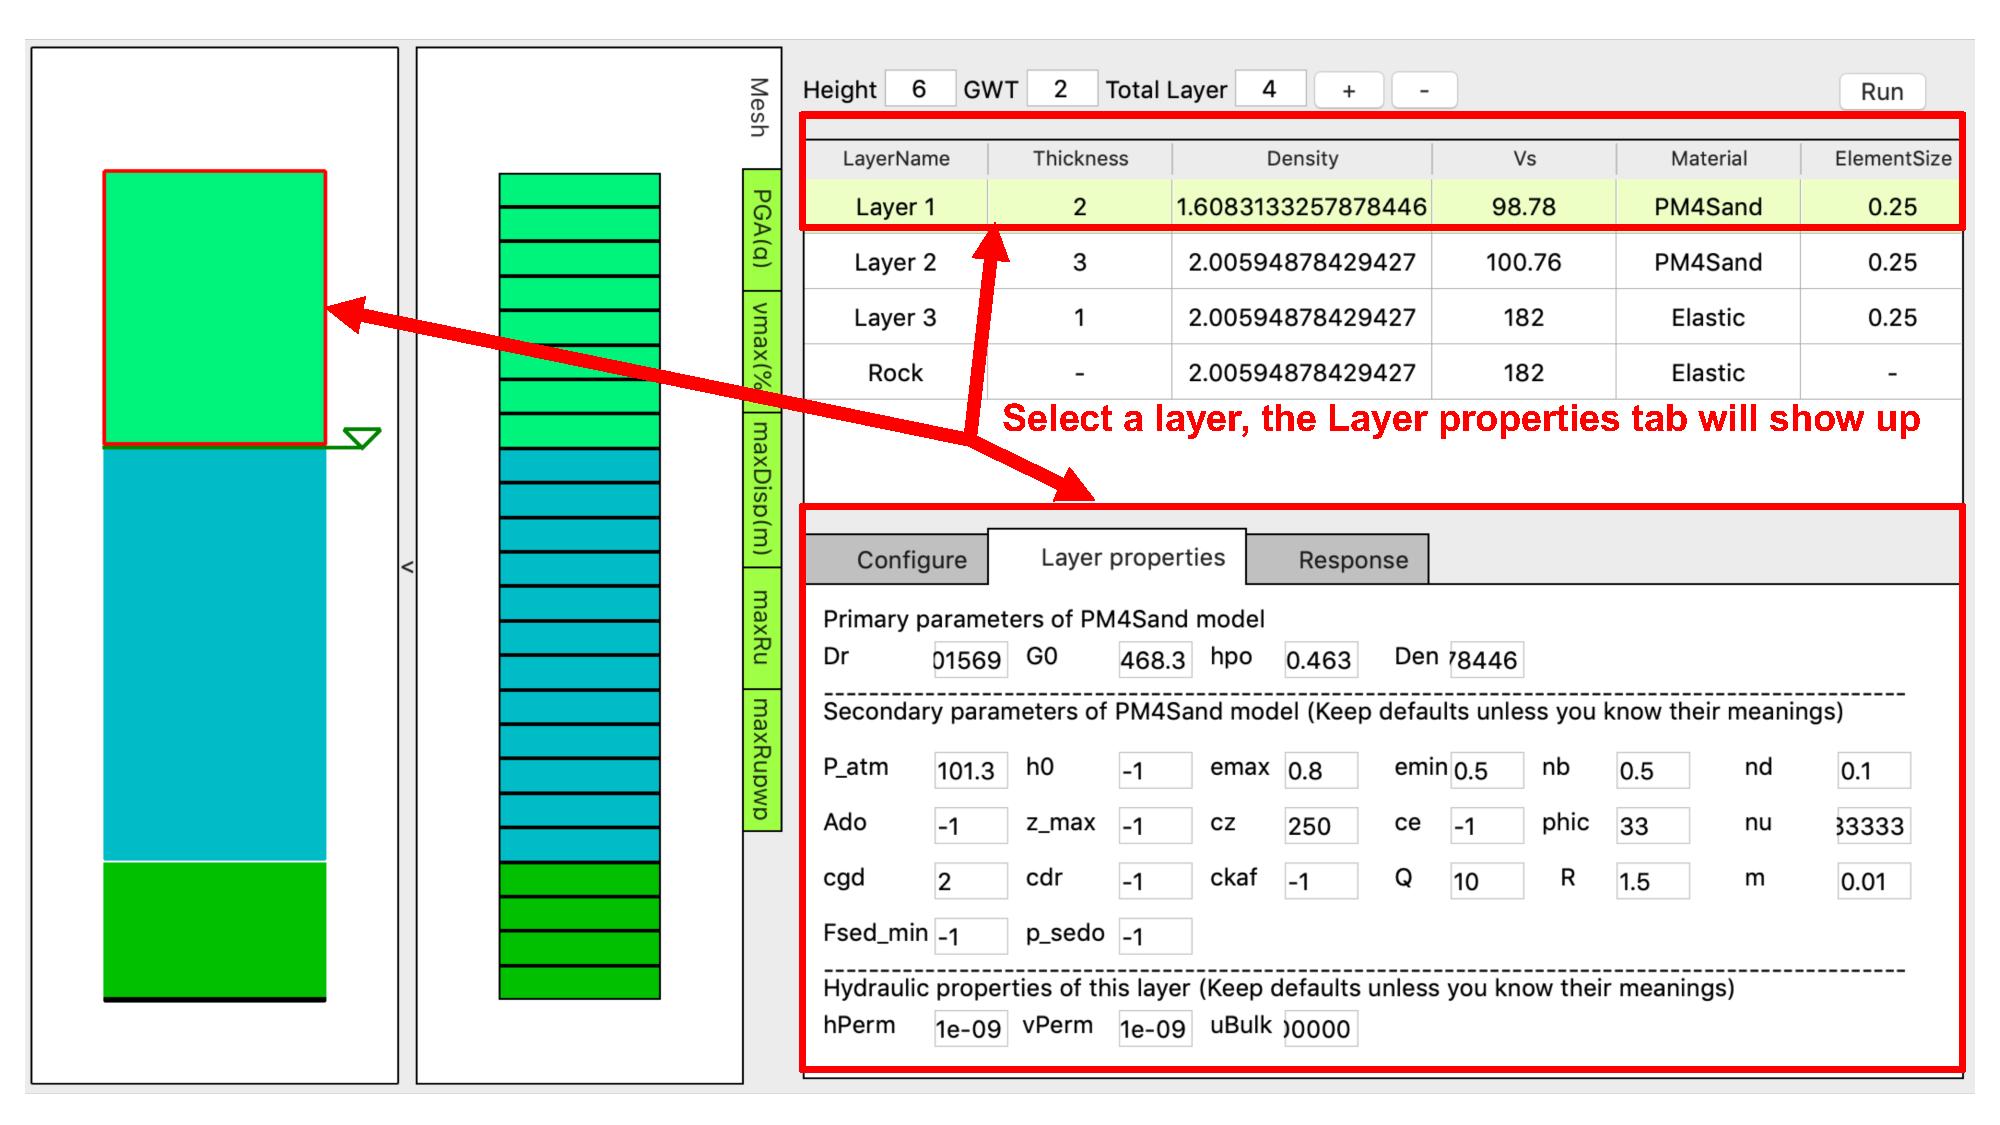
\includegraphics[width=0.8\textwidth]
    {usage/figures/s3hark3.pdf} }
  \caption{s$^3$hark - Layer modification }
  \label{fig:s3hark3}
\end{figure}


Upon the finish of the finite element analysis, the ground motion at the soil surface (\Cref{fig:s3hark4}) will be stored in EE-UQ's input file.
This computed motion will be later applied to the bottom of the building.

\begin{figure}[!htbp]
  \centering {
    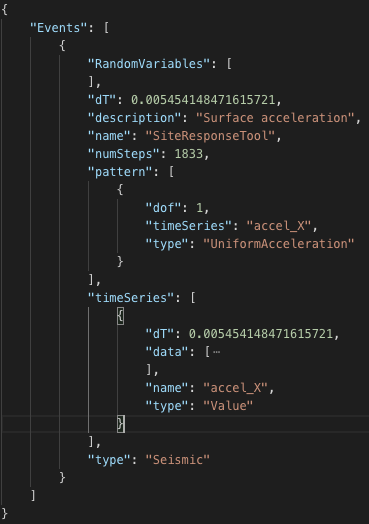
\includegraphics[width=0.4\textwidth]
    {usage/figures/s3hark4.png} }
  \caption{s$^3$hark - Surface motion }
  \label{fig:s3hark4}
\end{figure}


\subsection{User Application}
\label{subsec:user_event}
The final option for event definition is a user application. 
The user specifies the application name and the input file containing the specific input information 
needed by the application when it is running in the backend. 
As will be discussed later, when they use an additional application not provided, the user is also required 
to edit the tools registry file. There they must include a new event application with the same name 
and the location where that application can be found relative to the tools application directory. 
If running on DesignSafe, that application must be built and must be available on the Stampede2 supercomputer. 

Note: Given how DesignSafe runs the applications through Agave, the file permissions of this application must be 
world readable and executable (i.e., when a user runs their application through DesignSafe and Agave, they are not running it as themselves!)

\begin{figure}[!htbp]
  \centering {
    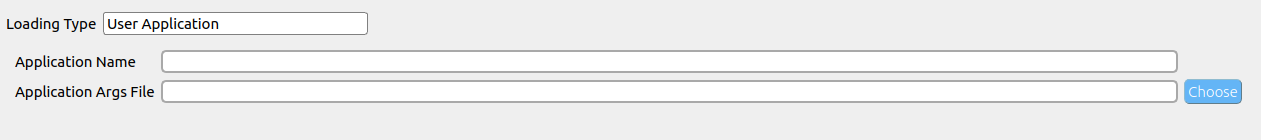
\includegraphics[width=1.0\textwidth]
    {usage/figures/userAppEvent.png} }
  \caption{User defined event}
  \label{fig:user_defined_event_panel}
\end{figure}


\subsection{PEER NGA Records}
\label{subsec:peer_nga_records}


This event allows the user to perform ground motion records selection and scaling using PEER NGA West 2 ground motions database. The suite of records can be selected from the database to represent the uncertainty in the ground motion. The following steps are needed to use this event:


\enumerate{
\item A target response spectrum must be specified by the user to be used for records selection and scaling.
\item The user specifies a selection criteria, such as the number of records and optional ranges of earthquake magnitude, distance to rupture (R\textsubscript{rup}) and shear wave velocity in the top 30 meter of soil (V\textsubscript{s}30).
\item The user run the record selection and inspect the selected suite of ground motions.
}


It is important to note that this event requires a PEER NGA West 2 account, users will be asked to provide their credentials (user name and password) to log in to the database. Users who do not have an account will be forwarded to the account sign up web page. Record selection is always done to minimize the mean square error between the target spectrum and the selected scaled spectrum. It is also important to note that the current version only allows user to specify the ASCE 7-10 design spectrum as a target. Future versions will allow the users to specify a user-provided target spectrum or a target spectrum obtained from seismic hazard analysis, such as the uniform hazard spectrum (UHS) or the conditional mean spectrum (CMS).


\begin{figure}[!htbp]
  \centering {
    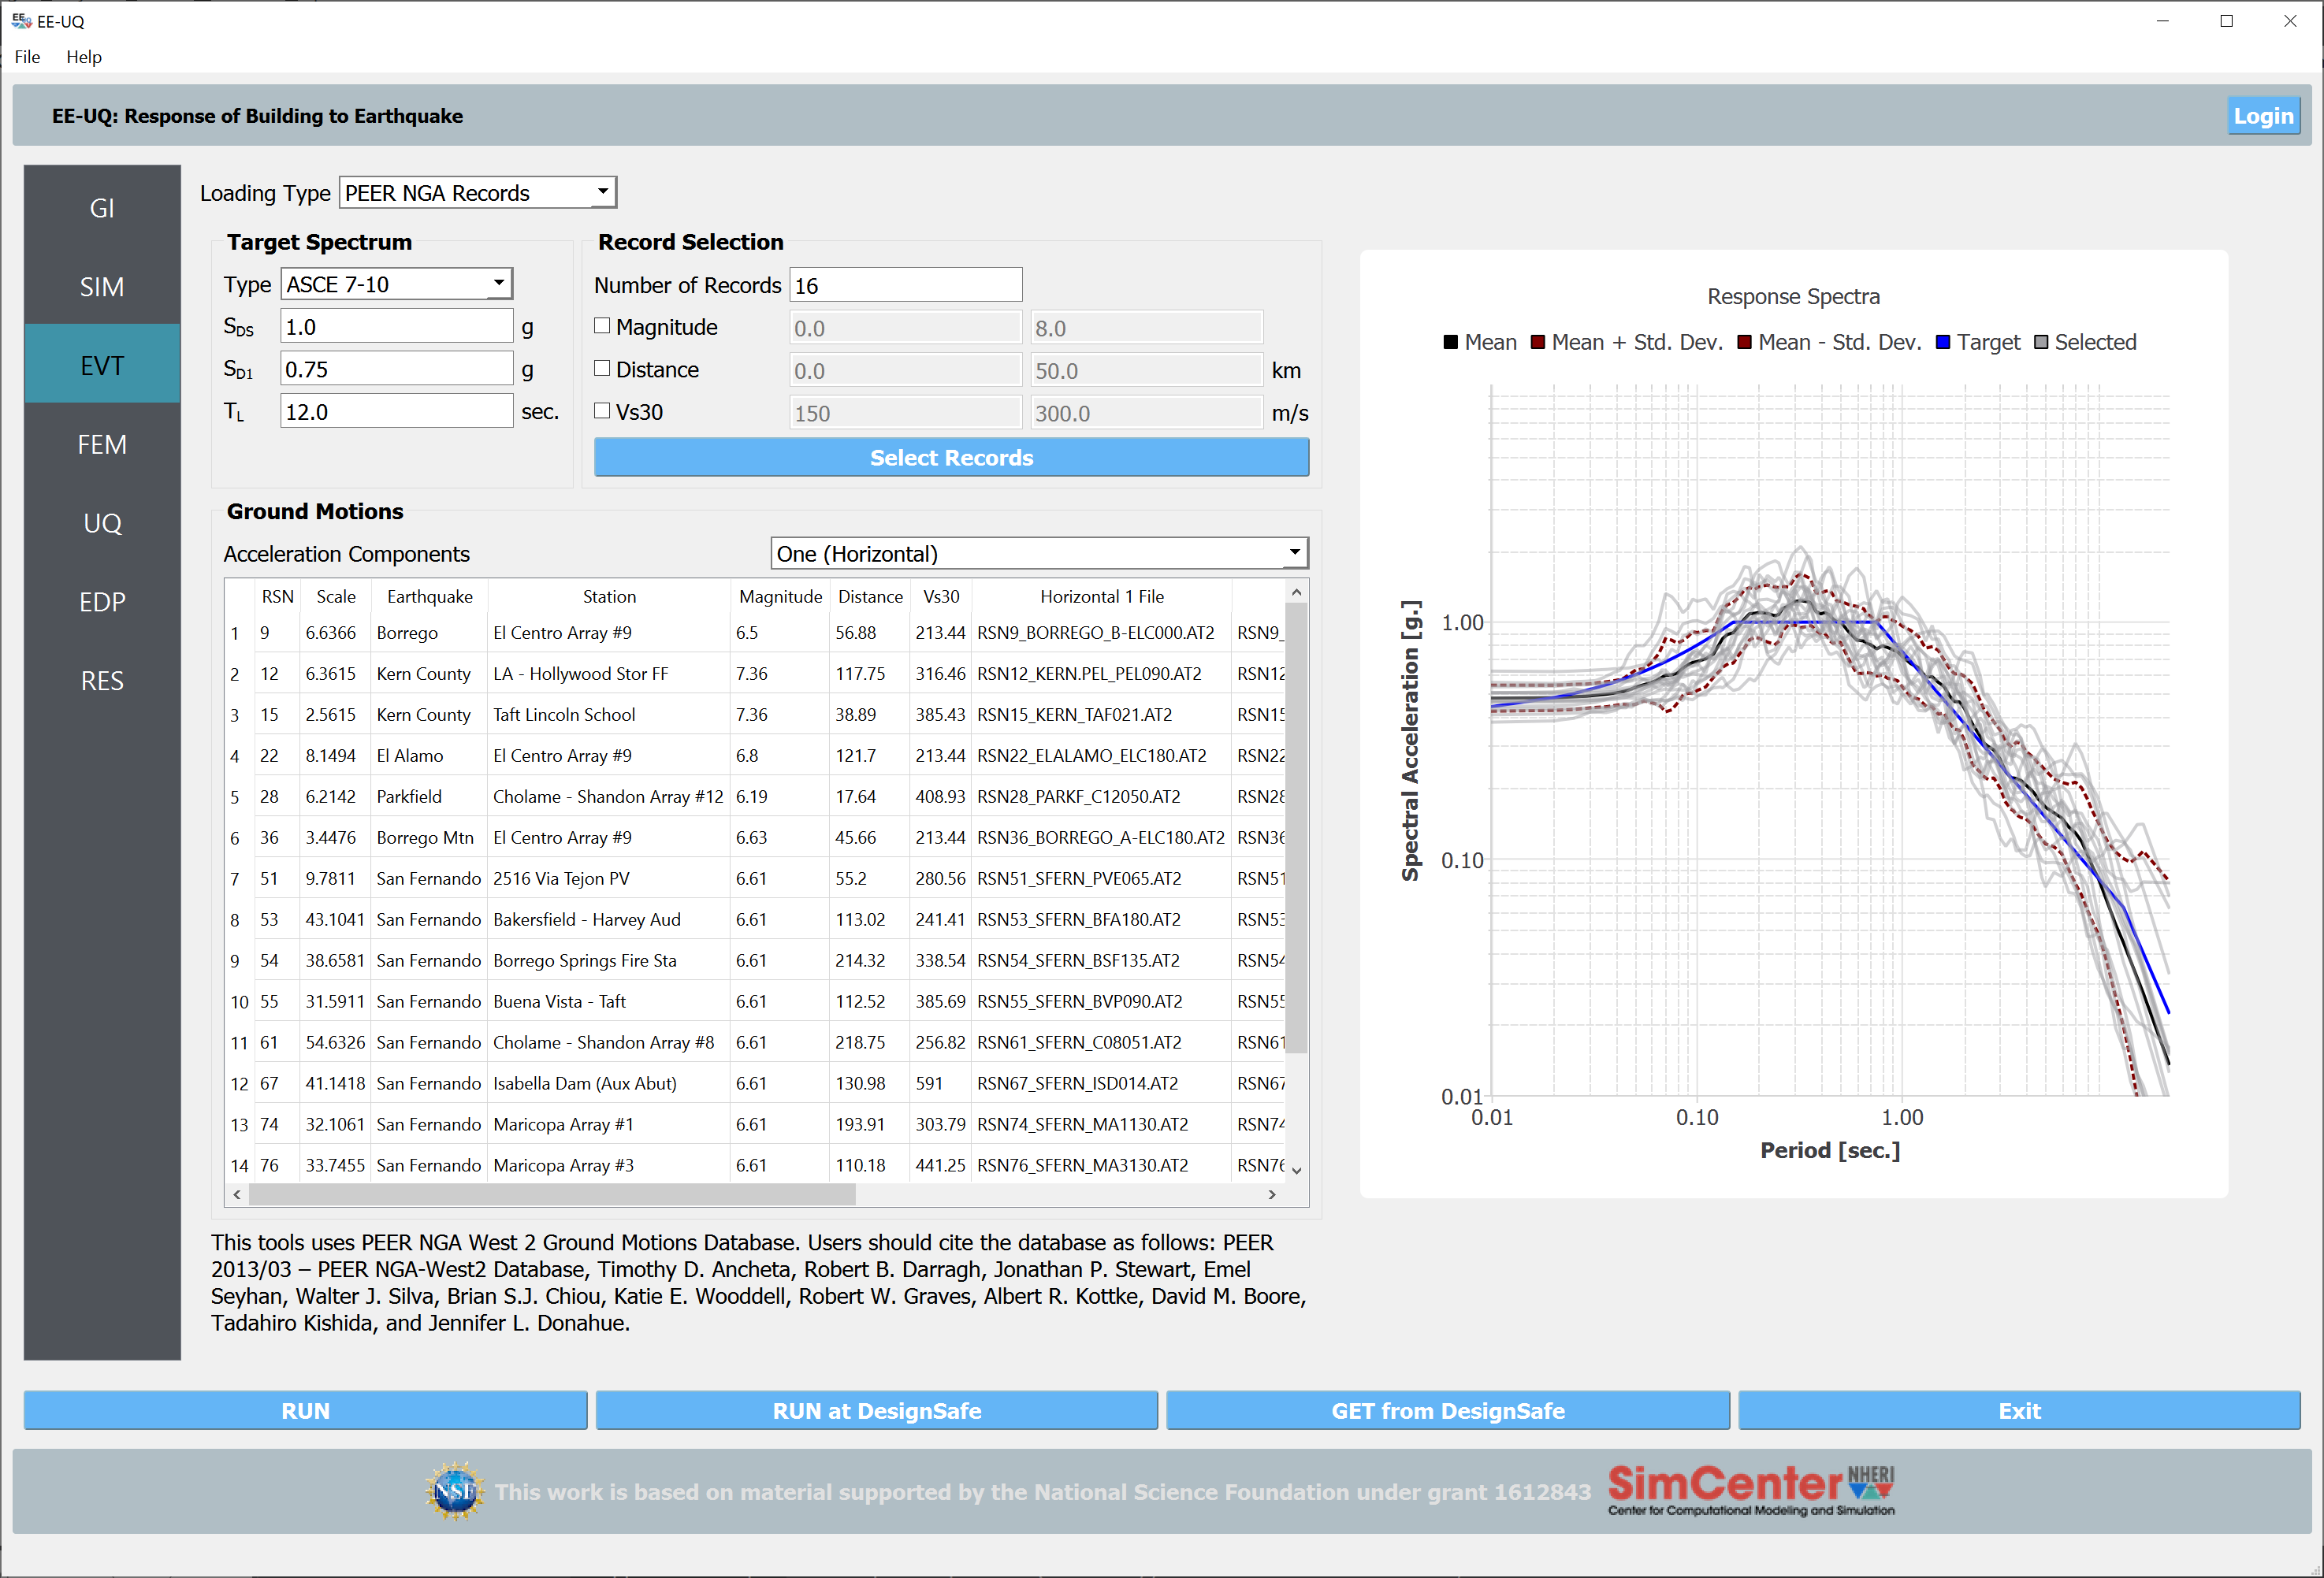
\includegraphics[width=0.8\textwidth]
    {usage/figures/PeerNgaRecords.png} }
  \caption{PEER NGA Records Event}
  \label{fig:PeerNgaRecordsWidget}
\end{figure}


After a suite of records is selected from the database, the list of records is shown in tabular form for the user to inspect their information, as shown in \Cref{fig:PeerNgaRecordsWidget}. Additionally a plot is generated showing the target spectrum, the average and standard deviation of the selected suite of records and the selected scaled ground motions spectra. Users can also highlight particular spectra on the plot by selecting the one or more records in the table provided. This enables the user to inspect the suite of records used to characterize the ground motions before running the building simulation.